\section{Overall Architecture and Main Module}
\label{sec:main}

BGPmon is divided into multiple modules.  The division into modules is driven by both conceptual and implementation 
objectives.   On a conceptual level,  BGPmon is designed to be extensible and it should be possible to enhance 
portions of BGPmon without modifying the entire code base.  For example, one may want to add new BGP capabilities or add new periodic reporting features or change the configuration of chains.   Our design separates the code into distinct modules so the code related to adding a new BGP capability is isolated in the peering module, to the maximum extent possible.   Similarly,  code related to periodic features would be in a periodic module and code related to chains configuration is in the chain module.    This modular design is intended to help facilitate additions at all levels.  

At an implementation level, the modules are designed to take maximum advantage of threading.    
Current trends in computer architecture are moving toward multi-core processors and threading programs can take maximum advantage of such designs.   Rather than attempt to micro-manage control, we allow the operating system to do this whenever possible. For example, we may be receiving data from multiple peers and not all of these peers will be sending data simultaneously.   Rather than building our own logic to select between peers, we launch a separate thread for each peer and rely on the operating system to fairly share resources among threads.        

\begin{figure*}
\centering
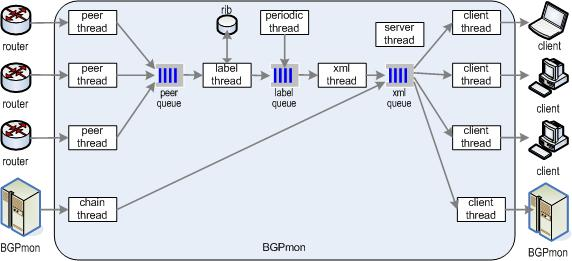
\includegraphics{figs/architecture.jpg}
\caption{BGPmon Architecture.}
\label{fig:architecture}
\end{figure*}

Figure \ref{fig:architecture} shows the overall system architecture and division into modules.

\subsection{Modules}

\emph{Configuration Module:}  provides the functions to read and save BGPmon configuration. These functions call module specific read/save configuration functions. Additionally, configuration module provides the XML unitlity functions which are needed by other modules. There is no threads associated with this module.

%This module launches all the main components and sets the overall rules for which peers are being monitored, what parameters to apply to each peer, what access procedures apply to clients,  which periodic
%events to announce and so forth.   A configuration is loaded at startup and then may be dynamically modified as the 
%BGPmon instance runs. 

\emph{Peering Module:}  
manages the conguration for all peers and one peering session for each enabled peer. 
The peer conguration could be changed by command line interface via interfaces provided by peering module. Peering session management includes opening the session, negotiating capabilities, monitoring the session state, receiving data from the session and reestablishing the session when needed. The BGPmon design allocates one thread for each peering session. All messages received from (and sent to ) a peer are written into the \emph{Peer queue} for processing by later modules.

%manages configurations for all peers and peering sessions for enabled peers.  The peer configuration could be changed be command line interface via interfaces provided by peering module.
%Peering session management includes opening the session, negotiating capabilities,  monitoring the session state,  receiving data from the session and reestablishing the session when needed.   
%The BGPmon design allocates one thread for each peering session.   All data received from (and sent to ) a peer are written into the \emph{Peer queue} for processing by later modules.

\emph{Labeling Module:}  manages one RIB-IN table associated with a peer if configured and uses the tables to assign labels to 
updates received from the peer.   The RIB tables may also be used by the periodic module discussed below.  Storage of RIB tables is optional and set by the administrator.   A single dedicated thread handles RIB tables and labeling for all peers.   The Labeling Module reads from the the \emph{Peer Queue} and writes to the \emph{Labeled Queue}.

\emph{Periodic Event Handling Module:}  manages periodic events such as requesting a route refresh from a peer and periodically 
announcing the status of peering sessions, queues and chains.  There are two threads in this module: one handles the route refreshes requests and another handles the periodic status messages.  By combining all periodic events in one place,  BGPmon can better manage events.   For example, the Periodic Module can stagger route refresh requests to large numbers of route table transfers do not occur at once.    Any messages written by the Periodic Module are placed into the \emph{Labeled Queue}.

\emph{XML Module:}  manages the conversion of all BGPmon received and generated messages into XML. 
A single dedicated thread handles all XML conversion.   The XML Module reads from the \emph{Labeled Queue} and writes to the \emph{XML Queue}.  

\emph{Clients Management Module:}  manages the server thread of BGPmon, accpeting connections from clients
and other BGPmons.   Once a connection is accepted, a distinct client thread is created for each client.     Client modules read from the \emph{XML Queue}

\emph{Chains Module:}  allows BGPmon instances to link together in a chain.    In the chain, the XML output of one BGPmon is fed directly into the XML queue of a second BGPmon instance.      For example one may deploy a BGPmon instance at an exchange point in London and deploy a second BGPmon instance at an exchange point in Amsterdam.   Both instances could chain to a third BGPmon in Oregon.    Clients that connect to the Oregon receive an XML stream that includes data from all three BGPmons.   The client is unaware BGPmons chains exist.    This chaining can later be combined with BGPbrokers who perform additional data processing tasks and produce a powerful monitoring network.    Any data received by the BGPmon Chains Module is written directly to the \emph{XML Queue}.
 
\emph{ Queue Module:}   handles the inevitable queuing issues that arise when bursty data sources provide real-time data to clients that accept data at different rates.    BGPmon implements queue management and pacing features that adjust clients who are too slow and attempt to pace bursts from routers so peering sessions are not dropped.
  
\emph{ Login Module:}   handles the Cisco-like commands typed by logined users and calls the corresponding functions provided by other modules.


\subsection{BGPmon Internal Format}
Messages are processed by various modules and flow through various queues until eventually being converted into an XML format and sent to clients as shown in Figure \ref{fig:architecture}.   For example, a BGP update is received by a peering thread,  placed in the \emph{Peer queue}, processed by the label thread and written into \emph{Labeled Queue} and finally read by the XML thread where the message is formated into XML and placed in the  \emph{XML Queue} that is forwarded to clients.    The periodic thread may also generate messages that are written into the \emph{Labeled Queue} directly.   All messages in the peer and label queues share a common BGPmon internal format shown in Figure \ref{fig:BMF}.    

\begin{figure}[!htb]
\centering
\scalebox{0.44}{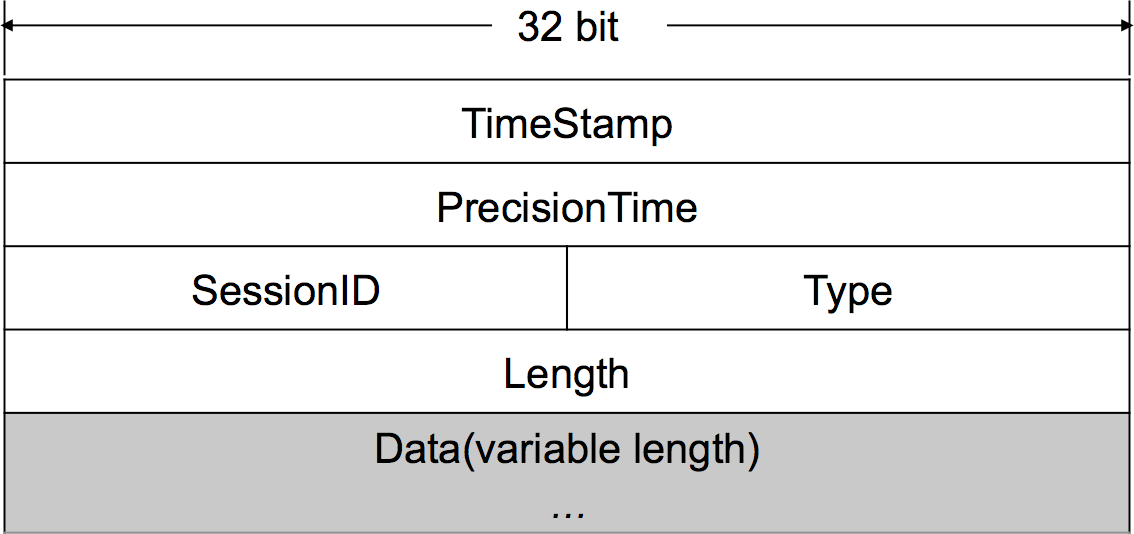
\includegraphics{figs/BMF.pdf}}
\caption{BGPmon Internal Format}
\label{fig:BMF}
\end{figure}
An internal format is needed to augment the data received from (or written to) the wire. The BGP messages received from peers do not carry a timestamp and the BGP message itself does not indicate the peering session over which it is received. BGPmon can easily add these information by recording the time and noting the corresponding peering session when the BGP message arrives. Similarly, messages generated by BGPmon also need to have a timestamp and are typically associated with some peering sessions. Rather than directly add timestamp and peering session information as XML tags, BGPmon dened an internal message format. The use of the internal format allows internal modules to operate on xed length binary elds for e?cient computations and centralizes all XML functions into one module. Any later changes to the XML standard are now conned to the single XML module.

%An internal format is needed to augment the data received from (or written to) the wire.   The BGP messages received from peers do not carry a timestamp and the BGP message itself does not identify the peer which sent the message.   BGPmon can easily add these values by recording the time at which a message was received and noting the peering session over which the data arrived.   Similarly, messages generated by BGPmon also need to have a timestamp and are typically associated with some peer.    Rather than directly add timestamp and peer data as XML tags, BGPmon defined an internal message format.     The use of the internal format allows internal modules to operate on fixed length binary fields for efficient computations and centralizes all XML functions into one module.    Any later changes to the XML standard are now confined to the single XML module. 
In BGPmon each peering session has a internal $SessionID$ and all peering sessions are indexed by $SessionID$. The Labeling module can use $SessionID$ to determine whether 
RIB tables and/or labels should be created for this peering session. The XML generation module can use the $SessionID$ to determine any necessary output information, ranging from the peers address and AS number to the number of bytes sent or received over this peering session.


%To identify the peer sending or receiving a message, BGPmon assigns its peering session a internal $SessionID$.   
%BGPmon maintains all peering sessions indexed by $SessionID$.    The Labeling module can use $SessionID$ to determine whether RIB tables and/or labels should be created for this peer.   The XML generation module can use the $SessionID$ to determine any necessary output information, ranging from the peer's address and AS number to the number of bytes sent or received from that peer.     

A small number of messages are not associated with any peering session and are assigned a $SessionID$ of zero in the internal format.   For example, control messages indicating BGPmon has started or is shutting down will have $SessionID = 0$.  

As the name implies, the internal format is strictly internal to a BGPmon instance.   Clients are never exposed to the BGPmon internal format.   Messages received from other BGPmon instances arrive already formated in XML and are placed directly into the XML queue as shown in Figure \ref{fig:architecture}.

A BGPmon Internal Format message consists of six fields shown in Figure  \ref{fig:BMF}.

\begin{itemize}
\item{\emph{TimeStamp:} is a 32 bit unix time stamp indicating when the message was received (for messages from peers) or generated (for messages sent by BGPmon).  }

\item{\emph{PrecisionTime:} is a 32 bit field indicating the number of microseconds and is used for more precise timing of messages, when the underlying operating system allows.}

\item{\emph{SessionID:} is a 16 bit number indicating the peering session over which the message was sent or received.  }   

\item{\emph{Type:} is a 16 bit number identifying the message type.    A listed of types is given in table \ref{tab:types}.}

\item{\emph{Length:} is a 32 bit number indicating the length of the data field in this message. }

\item{\emph{Data:} is a sequence of $Length$ octets and corresponds to the message itself.   }

\end{itemize}

\begin{figure*}
\centering
\begin{tabular}{| l | l | l |}
\hline
0 & Reserved & Reserved for future use \\
\hline
1 & BGPMsgSent  &  a BGP message generated by BGPmon and sent to a peer, generated by peering module\\
\hline
2 & BGPMsgRcvd & a BGP message received from a peer, generated by peering module\\
\hline
3 & BGPMsgLabeled &  a BGP message received from a peer and enhanced with labels, generated by labeling module\\
\hline
4  & BGPTableTransMsg &  updates reporting the RIB-IN table as part of a route refresh, generated by periodic module\\
\hline
5 & SessionStatus& instructs the XML module to report session status for a peer, generated by periodic module\\
\hline
6 & QueuesStatus& instructs the XML module to report  the status of all queues, generated by periodic module\\
\hline
7 & ChainsStatus& instructs the XML module to report the status of all chains, generated by periodic module\\
\hline
8 & FSMChange &  reports a transition in a peer's finite state machine, generated by peering module\\
\hline
9 & BGPMonStart &  a status message reporting BGPmon has started, generated by configuration module\\
\hline
10 & BGPMonEnd &  a status message reporting BGPmon is shutting down, generated by configuration module\\
\hline
\end{tabular}
\caption{BGPmon Internal Message Types}
\label{tab:types}
\end{figure*}
Note session ID in the message with type 6,7,9 and 10 is set to 0 as they are not specific to one peer.
 
%The BGPmon internal format must capture the time associated with a message 
%In order to facilitate the internal processing, we introduce the BGPmon internal formate: BMF. Simple stated, BMF adds a header to the incoming/outgoing BGP messages and state change messages. 
%
%\begin{verbatim}
%struct BGPmonInternalMessageFormatStruct
%{
%       struct OctetStruct
%        {
%        u_int32_t               timestamp;
%       u_int32_t               precisiontime;
%        u_int16_t               sessionID;
%        u_int16_t               type;
%        u_int32_t               length;
%        } header;
%        union BgpmonBodyStruct
%        {
%        	      struct OctetStruct
%                {
%                } Octet;
%                 struct StateChangeStruct
%                {
%                } state;
%                union MessagegeStruct
%                {
%                        struct OpenStruct
%                        {
%                        } open;
%                        struct UpdateStruct
%                        {
%                        } update;
%                        struct KeepaliveStruct
%                        {
%                        } keepalive;
%                        struct notificationStruct
%                        {
%                        } notify;
%                        struct OctetStruct
%                        {
%                        } octet;
%                } message;
%        } body;
%};
%\end{verbatim}
%
%We can easily extent this structure to support new types of internal messages. The reason I want to explicitly support the state change and BGP message here is multiple modules use them and we want to define them at one place.
%


%\subsection{Global Structures}

%BGPmon maintains several structures that are accessed by multiple modules.     These structures are used to share data between modules.   For example, the configuration module learns about peer information and must convey that information to the peering module that is responsible for opening the connection.    Similarly, the peering module maintains statistics on the number of messages received from a peer and must convey that information to the periodic module that reports peer status at regular intervals.      To facilitate this communication, several shared structures are used.     Although multiple modules may read from a structure,  the design attempts to ensure that every field in a structure has only one authorized writer.

%The \emph{Configuration Structure} holds all the configuration settings in format suitable for reading and writing XML configuration files and command line instructions.   It is created by the configuration module thread and is dynamically updated by the configuration thread as users modify the running configuration.    The Configuration Module is the only writer for this structure and generally only the configuration module reads this structure.    The structure is described further in Section \ref{sec:config}.

%The \emph{Peering Structure} holds all the information needed to manage a the connection with the peer and maintain statistics by the peer.   Each peer has its own session  structure, indexed by a $SessionID$.   It is created by the Configuration Module thread and then primarily maintained by a peering thread responsible for that peer.   After the thread has been created, some fields in this structure are written by the Configuration Module if a BGPmon administrator changes the peering configuration.    All other fields in this structure are written by the peering thread.    Readers of this structure include the Configuration Module to determine if configuration changes require reseting the peering session,  the Periodic Module to obtain statistics for reporting the status of a peer,  and the Labeling thread to manage the RIBIN table in some special circumstances.   The structure is described further in Section \ref{sec:peering}.

%The \emph{RIB and Labeling Structure} holds all the information needed to manage RIB-IN tables and assign labels to updates as specified by the configuration.   It is created by the Configuration Module thread and then be maintained by the RIB and Labeling Module thread.   After the thread has been created, some fields in this structure are written by the Configuration Module if a BGPmon administrator changes the RIB or labeling configuration.    Other fields in this structure are written by the RIB and labeling thread.    Readers of this structure include the Configuration Module to determine if configuration changes require reseting the RIB-IN or labeling rules, 
%the RIB and Labeling Module to manage the RIBIN and labels and the Periodic Module in cases when a peer does not support route refresh and RIBIN table must be periodically announced.  The structure is described further in Section \ref{sec:labeling}.

%The \emph{Periodic Events Structure}  holds all the information needed to manage periodic events as specified by the configuration.   It is created by the Configuration Module thread and then be maintained by the Periodic Events Module thread.   After the thread has been created, some fields in this structure are written by the Configuration Module if a BGPmon administrator changes the peering or periodic reporting configuration.    Other fields in this structure are written by the periodic events thread.    Readers of this structure include the Configuration Module to determine if configuration changes require reseting the periodic events and the Periodic Module to manage the events.    The structure is described further in Section \ref{sec:periodic}.

%The \emph{Clients Structure}  holds all the information needed to manage client connections.   It is created by the Configuration Module thread and then maintained by the client thread.   The structure is described further in Section \ref{sec:clients}.

%The \emph{BGPmon Chains Structure}  holds all the information needed to manage BGPmon chains as specified by the configuration.   It is created by the Configuration Module thread and then be maintained by the BGPmon Chains Module thread.   After the thread has been created, some fields in this structure are written by the Configuration Module if a BGPmon administrator changes the chaining configuration.    Other fields in this structure are written by the periodic events thread.    Readers of this structure include the Configuration Module to determine if configuration changes require reseting the chaining system and the BGPmon Chains thread to manage the events.    The structure is described further in Section \ref{sec:chains}.

%The \emph{Queueing Structure}  holds all the information needed to manage BGPmon queues.   It is created by the Configuration Module thread and then maintained by the queueing manager.   The structure is described further in Section \ref{sec:queue}.

%\item{Queue related Structure }
%\item{RIB/Labeling related Structure }
%\item{Server related Structure }


\subsection{The Startup and Main Program}

\subsubsection{Parse Command Line Arguments}
The main program starts with parsing the command line arguments.   Currently there are only a few simple command line arguments.    First,  a configuration file name can be provided using the \emph{-c filename}.   The configuration file, discussed in more detail in section \ref{sec:config}, provides essential information ranging from the ports to listen for connections,  the peers to monitor, and so forth.    If no configuration file is specified, a default configuration file name specified in \emph{site\_defaults.h} will be used. 

The \emph{-r port} instructs BGPmon to start the Command Line Interface on the recovery port.  The recovery port is discussed later in section  \ref{sec:main:design} .%The Command Line Interface port can also be specified in the Configuration File.     
%If a user sets both the \emph{-r port} option and configures a port in the Configuration File, then the Configuration File takes precedence and the  \emph{-r port} option is ignored. 

The remaining optional command line arguments sets the logging functions.    The program can be set to run in an interactive mode that sends all messages to stdout using the \emph{-i} option.    Alternately, the program can be set to log all messages using syslog using the \emph{-s} option.    The \emph{-i} and \emph{-s} options are mutually exclusive and the program exits with an error if both are specified.    If neither option is specified,  a default value is built into the code and specified in Util/log.h.     

The \emph{-l loglevel} option specifies the log level and uses the standard syslog values as follows.    Emergencies, Alerts, Critical Errors, and Errors are levels 0 to 3 (respectively).    These messages are always logged regardless of the log level setting.    Warnings, Notices, Information, and Debug output are levels 4 to 7 (respectively).   Setting $loglevel = L$ will log all messages at and below the $L$.   For example, a log level of 4 will display Alerts, Critical Errors, Errors, and Warnings, but will not display Notices, Information, or Debugging output.     If the \emph{-l loglevel} option is not specified,  a default logvalue is built into the code and specified in Util/log.h.   {\bf For full debug output,   compile with DEBUG set to 1.}

If messages are logged to syslog, the syslog Facility can be set with the \emph{-f facility} option.    If the \emph{-f facility} option is not specified,  a default syslog facility is built into the code and specified in Util/log.h.     This option has no effect if messages are written to standard output (e.g. if \emph{-i} was specified).    

\subsubsection{Read Configuration File}
After parsing the command line, the main program initialize the settings of all other modules by calling per-module specific initialization function. This needs to be done before reading configuration file.
Then it continues to read the configuration file by calling the facade function "readConfigFile" provided by configuration module. 
If the configuration file is corrupted or not readable, main program will first backup the corrupted file by calling "backupConfigFile" and then try to save as much as it can by calling "saveConfigFile". The new saved configuration file is readable and a part of corrupted one. After that, BGPmon will exit.
If no configuration file is existing, main program will go ahead to start other threads and simply waits for the user to configure BGPmon via command line interface.


\subsubsection{Launch and Monitor Other Threads}
After reading conguration les, main program launches all other threads including peer threads, labeling thread, XML thread, periodic thread, clients management thread, chains threads, login thread and signal handling thread. 
As BGPmon could be running for a long time, it is likely some threads get hang or die. If one critical thread dies, the entire BGP wont work correctly. So main program also needs to make sure all the threads are still alive. Specically, each thread keeps updating a timestamp to indicate its aliveness and main program keeps checking the timestamp of each module. If one timestamp hasnt been updated for THREAD\_CHECK\_INTERVAL, main thread will infer the corresponding thread died. That also requires every module needs to make sure its threads update their timestamps at least once per THREAD\_CHECK\_INTERVAL. BGPmon will also exit gracefully upon receipt of an interrupt signal. All signal processing and shutdown procedures are handled by the signal handling thread. 

%After reading configuration files, main program launches all other threads including peer threads, labeling thread, XML thread, peridoic thread, clients management thread, chains threads, login thread and signal handling thread.
%It also monitor these threads to make sure if they are still active. Specifically, each thread keeps updating a timestamp to indicate its aliveness and main thread keeps checking the aliveness flag of each module. If one flag hasn't
%been updated for a particular interval, main thread will infer the corresponding thread died. 
% BGPmon will also close gracefully upon receipt of an interrupt signal.  All signal processing and shutdown procedures are handled by the signal handling thread.
 
 \subsection{Design Philosophy}
 \label{sec:main:design}
Besides the design issues mentioned above such as modular architecture and internal message format, how to congure BGPmon is another critical design issue. If we dont design it carefully and make the learning curve low, it would be very di?cult to be deployed widely in the operational community. In the previous design, BGPmon used to be congured by manually editing a XML conguration le. Then we found 2 main issues of this approach: 
 \begin{itemize}
	 	\item{ The configuration of BGPmon could be complex if there are hundreds of peers. That means editing configuration file manually could be tedious and error-prone.}
		\item{ Learning the format of conguration le would be a barrier of using BGPmon.  }
\end{itemize} 

In order to address these 2 issues, we decided to mimic cisco IOS conguration. Specically, everything is congured via command line interface which is a telnet client typically. All the conguration via command line interface can be saved in a le and normal users are unaware of the existence of this le just like a cisco router. But the only di?erence is expert users have the exibility to save multiple conguration les and switch among them in BGPmon . By doing this, the learning curve will be less steeper especially for those who are familiar with cisco IOS conguration.

As the conguration le is not supposed to be edit manually by normal users, it shouldnt be corrupted unless hardware errors, BGPmons bugs and edition by expert users. But even now the probability of having a corrupted
conguration le is low, we still need to design a failover mechanism in case of corruption. In our current design, if the conguration le gets corrupted,
 \begin{itemize}
	 	\item{ First, the corrupted conguration le is backed up.}
		\item{Secondly, BGPmon tries to save as many parts as possible into a new conguration le.}
		\item{ At last, BGPmon exits to alert users the corruption of conguration le.}
\end{itemize} 

We now argue why those actions are necessary. If BGPmon just quits without saving a new readable conguration le, the user has to manually x the corrupted le. With a new conguration le, the user can restart 
the BGPmon easily. And we dont want to just delete the corrupted le either as it is not acceptable all other peers conguration get lost only because of the corruption of rst peers conguration. 
The backed up corrupted le is mainly for the expert users to gure out the problem. Our aim here is to avoid loss of conguration and manual x in case of corruption.

Last but not least, BGPmon typically listens on a default or congured port for conguration via command line interfaces. 
But in the following 2 cases, the recovery port( -r port ) option is needed to start a BGPmon.
 \begin{itemize}
	 	\item{ The default port is in use when BGPmon starts for the rst time, specially if you dont want to change the default conguration and recompile BGPmon. }
		\item{ The congured port is blocked by misconguring the access control. Then no one can change the access control list via command line interface as the congured port is blocked. 
				With recvoery port, administrator could restart BGPmon with a non-blocked port and use command line interface to correct the misconguration. }
\end{itemize} 
% \begin{itemize}
% 	\item{\emph{ BGPmon configuration:}  BGPmon configuration is very similar to cisco IOS configuration. Basically everything is configured via command line interface which is telnet client typically.  All the configurations via command line interface are stored in a XML file. But most users are unaware of the existence of this file except expert users. Expert users can have multiple configuration files and switch among them by using the \emph{-c filename}.
%	There are 2 reasons of imitating cisco IOS configuration:
%	 \begin{itemize}
%	 	\item{ The configuration of BGPmon could be complex if there are hundreds of peers. That means editing configuration file manually could be tedious and error-prone.}
%		\item{ It would be easy to learn BGPmon configuration for the users who are familiar with cisco IOS configuration.  }
%	\end{itemize} 
%	}
% 	\item{\emph{ Default configuration:}  The default configuration of BGPmon can be found in site\_defaults.h. It can be changed by editing this file and then recompile BGPmon. There are 2 reasons why we need this default configuration.
%		 \begin{itemize}
%	 	\item{ It includes all the needed configurations to start BGPmon for this first time. For example, the command line interface needs a default enable password and a default port to listen on even if there is no configuration yet.  }
%		\item{ It provides the defaults for all the optional configurations. For example, the BGP version of peer configuration is optional and the default value will be used if it is not specified by the user.    }
%	\end{itemize} 
%	Default configuration will be overwritten by the configuration via command line interface.
%	}
%		
% 	\item{\emph{ Corrupted configuration file:}  As the configuration file is not supposed to be edit by normal users, it shouldn't be corrupted unless hardware errors, BGPmon's bugs and edition by expert users. If it is corrupted,  we first backup the corrupted configuration file, then save as many parts as possible into a new configuration file and quit BGPmon at last.  If BGPmon just quits without saving a new readable configuration file, the user has to manually fix the corrupted file. With a new configuration file, the user can restart the BGPmon easily. And we don't want to just delete the corrupted file either as it is not acceptable all other peers' configuration get lost only because of the corruption of first peer's configuration. The backed up corrupted file is mainly for the expert users to figure out the problem.
%Our design philosophy here is to avoid the loss of configuration and the manual fix in case of corruption. }

%	\item{\emph{ Recovery port( \emph{-r port}) of command line interface:} The recovery port option is needed if the default port is in use when BGPmon starts for the first time, specially if you don't want to change the default configuration and recompile BGPmon. It is also important when the configured port is blocked by misconfiguring the access control list. Usually command line interface listens on the configured port.						But administrator may misconfigure the access control list to block the configured port.  Then no one can change the access control list via command line interface as the configured port is blocked. 
%					With recvoery port, administrator could restart BGPmon with a non-blocked port and use command line interface to correct the misconfiguration. }
%	\item{\emph{ Check aliveness of threads:} As BGPmon could be running for a long time, it is likely some threads get hang or die. If one critical thread dies, the entire BGP won't work correctly. So we need to make sure all the threads are still running. As main program checks the aliveness flag every\\* THREAD\_CHECK\_INTERVAL,  every module needs to make sure its threads update their aliveness flags at least once per THREAD\_CHECK\_INTERVAL. }
%	
%\end{itemize} 




%\begin{verbatim}
%main()
%{
%	/*Parse the configuration file and return a struct 
%	 * which includes the following things:
%	* 1. Configuration Structure - cs, 
%	* 2. Periodic Events Structure - pes
%	* 3. A part of Session Structure - ss 
%	* 4. Queue related Structure - qs
%	* 5. RIB/Labeling related Structure - rs
%	* 6. Server related Structure - ss
%	* 7. BGPmon chain related Structure - cs
%	*/
%	CONFIG cfg = configurationParser(configurationFileName);
%
%	/*Create 3 queues: monitor queue, label queue 
%	 *and xml queue
%	 */
%	QueueConfig qc = cfg.qc;
%	Queue mq = createMonitorQueue(qc);
%	Queue lq = createLabelQueue(qc);
%	Queue xq = createXMLQueue(qc);
%	
%	/*Start peering threads, one for each peer*/
%	PeerSessions ps = CreatePeeringSessions(cfg.SS, mq);
%	for each peer p in ps
%	{
%		startPeeringThead(p);
%	}
%	
%	/*Start RIB/Labeling thread if needed*/
%	RIBConfig rc= cfg.rc;
%	startRIBLabelThread(rc, mq, lq);
%	
%	/*Start XML thread*/
%	startRIBLabelThread(lq, xq);
%	
%	/*Start BGPmon chain thread*/
%	ChainConfig cc = cfg.cc;
%	startChainThread(cc);
%		
%	/*Start periodic events thread*/
%	PES pes = cfg.pes;
%	startPeriodicEventsThread(pes);
%			
%	/*Start command line thread*/
%	CS cs = cfg.cs;
%	startCommandlLineThread(cs, ps, pes, cc, ....);
%	
%	/*Start signal handler thread*/
%	startSignalHandlerThread( );	
%	
%	/*Start server thread, there is a permanent loop inside*/
%	ServerConfig sc = cfg.sc;
%	startSeverThread(sc);	
%}
%\end{verbatim}  
